\documentclass[12pt]{article}

\usepackage[utf8]{inputenc}
\usepackage{latexsym,amsfonts,amssymb,amsthm,amsmath}
\usepackage{float}

\setlength{\parindent}{0in}
\setlength{\oddsidemargin}{0in}
\setlength{\textwidth}{6.5in}
\setlength{\textheight}{8.8in}
\setlength{\topmargin}{0in}
\setlength{\headheight}{18pt}
\usepackage{graphicx}
\usepackage{tikz}

\usepackage{hyperref}
\hypersetup{
    colorlinks=true,
    linkcolor=blue,
    filecolor=magenta,      
    urlcolor=cyan,
    pdftitle={Overleaf Example},
    pdfpagemode=FullScreen,
}

\urlstyle{same}

\usepackage{caption}
\DeclareCaptionFormat{citation}{%
  \ifx\captioncitation\relax\relax\else
    \captioncitation\par
  \fi
  #1#2#3\par}
\newcommand*\setcaptioncitation[1]{\def\captioncitation{\textit{Source:}~#1}}
\let\captioncitation\relax
\captionsetup{format=citation,justification=centering}

\title{MATH1034OL1 Pre-Calculus Mathematics Notes from Sections 4.7, 3.2 (Monday)}
\author{Elijah Renner}

\begin{document}

\maketitle

\vspace{0.5in}

\tableofcontents

\section{Identities}

\subsection{Pythagorean Identities}

We first derive the identity \(\cos^2\theta + \sin^2\theta = 1\) from the unit circle.\\

\begin{figure}[H]
	\centering
	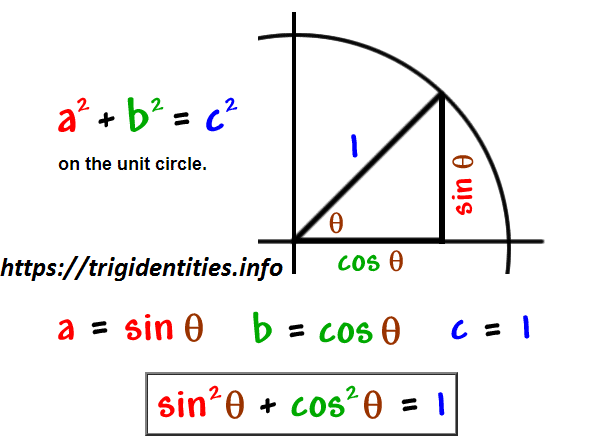
\includegraphics[scale=0.4]{Pythagorean Identity.png}
	\caption{Credit: \url{https://trigidentities.info/pythagorean-trig-identities/}}
\end{figure}

Then, the other two Pythagorean identities are derived by dividing by either \(\cos^2\) or \(\sin^2\):\\

To derive \(\tan^2\theta+1=\sec^2\theta\), divide the original identity by \(\cos^2\theta\):\\

\[\frac{\cos^2\theta + \sin^2\theta = 1}{\cos^2\theta}\implies\frac{\cos^2\theta}{\cos^2\theta}+\frac{\sin^2\theta}{\cos^2\theta}=\frac{1}{\cos^2\theta}\implies\tan^2\theta+1=\sec^2\theta\]

To derive \(\cot^2\theta+1=\csc^2\theta\), divide the original identity by \(\sin^2\theta\):\\

\[\frac{\cos^2\theta + \sin^2\theta = 1}{\sin^2\theta}\implies\frac{\cos^2\theta}{\sin^2\theta}+\frac{\sin^2\theta}{\sin^2\theta}=\frac{1}{\sin^2\theta}\implies\cot^2\theta+1=\csc^2\theta\]

To summarize, the three Pythagorean identities are 

\begin{enumerate}
	\item \(\cos^2\theta + \sin^2\theta = 1\)
	\item \(\tan^2\theta+1=\sec^2\theta\)
	\item  \(\cot^2\theta+1=\csc^2\theta\)
\end{enumerate}

\subsection{Sum and Difference Formulas}

The sum and difference formulas allow us to evaluate the trigonometric functions of angles whos reference angles aren't 30, 45, 60, or 90:\\

\[\sin(A\pm B)=\sin A\cdot\cos B \pm \cos A\cdot\sin B\]

\[\cos(A\pm B)=\cos A\cdot\cos B \mp \sin A\cdot\sin B\]

There is a formula for \(\tan(A\pm B)\), which isn't necessary to remember, as it can be derived from \(\frac{\sin(A\pm B)}{\cos(A\pm B)}\) since \(\tan\theta=\frac{\sin\theta}{\cos\theta}\). The same follows for \(\csc(A\pm B)=\frac{1}{\sin(A\pm B)}\), \(\sec(A\pm B)=\frac{1}{\csc(A\pm B)}\), and \(\cot(A\pm B)=\frac{\cos(A\pm B)}{\sin(A\pm B)}\).\\

Regardless, \\

\[\tan(A\pm B)=\frac{\tan A\pm \tan B}{1\mp\tan A\cdot\tan B}\].

Also, \(\mp\) indicates the opposite sign of whichever sign is chosen as \(\pm\).

\subsection{Double Angle Formulas}

To derive the double angle formulas, we start with the angle familiar sum identities.

\subsubsection{Sine}

The angle sum identity for sine is:
\[
\sin(A + B) = \sin A \cos B + \cos A \sin B
\]

By setting \(A = B = \theta\), we get:
\[
\sin(2\theta) = \sin(\theta + \theta) = \sin \theta \cos \theta + \cos \theta \sin \theta
\]

Simplify this by combining like terms:
\[
\sin(2\theta) = 2 \sin \theta \cos \theta
\]

\subsubsection{Cosine}

The angle sum identity for cosine is:
\[
\cos(A + B) = \cos A \cos B - \sin A \sin B
\]

By setting \(A = B = \theta\), we get:
\[
\cos(2\theta) = \cos(\theta + \theta) = \cos \theta \cos \theta - \sin \theta \sin \theta
\]

Simplify this by combining like terms:
\[
\cos(2\theta) = \cos^2 \theta - \sin^2 \theta
\]

Using the Pythagorean identity \(\sin^2 \theta + \cos^2 \theta = 1\), we can derive alternative forms of \(\cos(2\theta)\):\\

1. Express \(\cos^2 \theta\) in terms of \(\sin^2 \theta\):
\[
\cos^2 \theta = 1 - \sin^2 \theta
\]

Substitute this into the double angle formula for cosine:
\[
\cos(2\theta) = (1 - \sin^2 \theta) - \sin^2 \theta = 1 - 2 \sin^2 \theta
\]

2. Express \(\sin^2 \theta\) in terms of \(\cos^2 \theta\):
\[
\sin^2 \theta = 1 - \cos^2 \theta
\]

Substitute this into the double angle formula for cosine:
\[
\cos(2\theta) = \cos^2 \theta - (1 - \cos^2 \theta) = 2 \cos^2 \theta - 1
\]

So, we have three equivalent forms of \(\cos(2\theta)\):
\[
\cos(2\theta) = \cos^2 \theta - \sin^2 \theta = 1 - 2 \sin^2 \theta = 2 \cos^2 \theta - 1
\]

These derivations give us the double angle formulas for sine and cosine:
\[
\sin(2\theta) = 2 \sin \theta \cos \theta
\]

\begin{align*}
\cos(2\theta) &= \cos^2 \theta - \sin^2 \theta \\
  &= 1 - 2 \sin^2 \theta \\
  &= 2 \cos^2 \theta - 1
\end{align*}


Nice!

\subsection{Half Angle Formulas}

The half angle formulas for \(\sin\) and \(\cos\) are\\
  
\[
\sin^2\theta = \frac{1}{2}(1 - \cos(2\theta)) \implies \sin\theta = \pm \sqrt{\frac{1}{2}\left(1 - \cos(2\theta)\right)} = \pm \sqrt{\frac{1 - \cos(2\theta)}{2}}
\]

\[
\cos^2\theta = \frac{1}{2}(1 + \cos(2\theta)) \implies \cos\theta = \pm \sqrt{\frac{1}{2}\left(1 + \cos(2\theta)\right)} = \pm \sqrt{\frac{1 + \cos(2\theta)}{2}}
\]\\

To derive the half-angle formula for \(\tan\), we use the half-angle formulas for \(\sin\) and \(\cos\):
\[
\tan \theta = \frac{\sin \theta}{\cos \theta}
\]

Using the half-angle formulas:
\[
\sin \theta = \pm \sqrt{\frac{1 - \cos(2\theta)}{2}}
\]
\[
\cos \theta = \pm \sqrt{\frac{1 + \cos(2\theta)}{2}}
\]

So,
\[
\tan \theta = \frac{\sin \theta}{\cos \theta} = \frac{\pm \sqrt{\frac{1 - \cos(2\theta)}{2}}}{\pm \sqrt{\frac{1 + \cos(2\theta)}{2}}}
\]

Since both the numerator and the denominator have the same sign, the signs cancel out:
\[
\tan \theta = \sqrt{\frac{1 - \cos(2\theta)}{2}} \div \sqrt{\frac{1 + \cos(2\theta)}{2}} = \sqrt{\frac{1 - \cos(2\theta)}{1 + \cos(2\theta)}}
\]

Thus, the half-angle formula for \(\tan\) is:
\[
\tan \theta = \sqrt{\frac{1 - \cos(2\theta)}{1 + \cos(2\theta)}}
\]

\subsection{Quizlet}

I know that was a lot. There's a lot to remember, so I'll be quizzing myself. Here is my quizlet:\\

\href{https://quizlet.com/928964860/precalculus-identities-flash-cards/?funnelUUID=024bad64-6810-4a54-bcac-a822e71b26c7}{Quizlet Link}\\

You might bookmark this, since I'll be updating it as we learn more identities.\\

\section{Vertex of Quadratic}

Let \(f(x)=ax^2+bx+c\) where \(a\), \(b\), and \(c\) are constants. The vertex of \(f\) will always be\\

\[\left(\frac{-b}{2a}, f\left(\frac{-b}{2a}\right)\right)\]

\section{Polynomial Behavior}

If a factor \((x-a)\) appears an even amount of times, the function will touch the x-axis when \(x=a\).\\

Conversely, if \((x-a)\) appears an odd amount of times, the function will cross the x-axis when \(x=a\):

\begin{figure}[H]
	\centering
	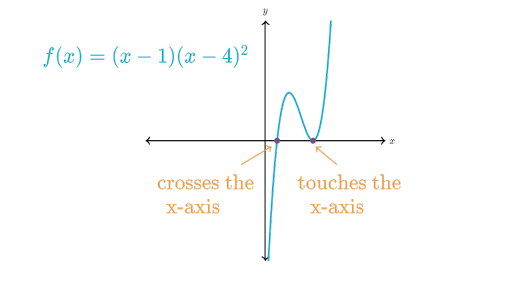
\includegraphics[scale=1]{Polynomial touching.png}
	\caption{Credit: \url{https://www.khanacademy.org/math/algebra2/x2ec2f6f830c9fb89:poly-graphs/x2ec2f6f830c9fb89:poly-intervals/a/zeros-of-polynomials-and-their-graphs}}
\end{figure}

In class, we reviewed the end behaviors of polynomials. I've already recorded them in the notes from July 5th. Good luck on Friday!

\end{document}